
\chapter{Phased Gated Recurrent Units Network}
In this chapter, the goal is to introduce the theoretical structure of the conversion predictor that we are training. 
Neural networks are very popular as they can be used for regression and classification tasks, achieve reliably good results, and there are several ways to customize them to boost their performance even further.   \\
We start with an introduction of basic neural networks before discussing recurrent neural networks (RNN) to help build an intuition for the GRU network we want to use as the conversion predictor. 
Finally, the addition and functionality of a so-called time gate in the phased GRU Cell, which we use to handle the non-uniform time intervals between touchpoints is explained.

\section{Neural Networks}

To lay the necessary foundation and introduce a common notation we first consider basic neural networks. \\
The idea behind neural networks stems from the idea of how information is processed by neurons in the human brain, where neurons collect and process incoming information and distribute their outcome to other neurons. \\
Mathematically we model \textit{neurons} as follows:

\begin{figure}[h]
\centering
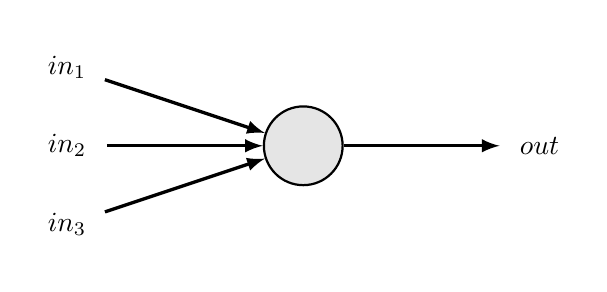
\begin{tikzpicture}[item/.style = {circle, draw, thick, align = center},
itemc/.style = {item, join}]

\node[circle, minimum size = 10mm, fill = white] (i-1) at (0,0) {$in_1$};
\node[circle, minimum size = 10mm, fill = white] (i-2) at (0, -1){$in_2$};
\node[circle, minimum size = 10mm, fill = white] (i-3) at (0, -2){$in_3$};
\node[item, minimum size = 10mm, fill = gray!20] (h1) at (3, -1) {$ $};
\node[circle, minimum size = 10mm, fill = white ] (o) at (6, -1) {$out$};

% Connect neurons 
\draw[-latex,very thick] (i-1) -- (h1);
\draw[-latex,very thick] (i-2) -- (h1);
\draw[-latex,very thick] (i-3) -- (h1);
\draw[-latex,very thick] (h1) -- (o);

\end{tikzpicture}
\label{abb:neuron}
\caption{Neuron}
\end{figure}

In picture \ref{abb:neuron} an example neuron is depicted, that is taking three input values $in_1, in_2, in_3 \in \R$ and transforming them to an output value $out\in \R$, by performing a linear transformation and then applying an activation function. The linear transformation consists of multiplying the input values using three weights $w_1, w_2, w_3\in \R$ and adding a bias value $b\in \R$ and then applying an activation function $\sigma$.
\begin{align*}
    out& = \sigma(w_1 \cdot in_1 + w_2 \cdot in_2 + w_3\cdot in_3 + b)\\
    & = \sigma(w^T in + b),
\end{align*}
with $in=(in_1,in_2,in_3)^T\in\R^3$ and $w=(w_1,w_2,w_3)^T\in\R^3$.\\
More general:
\begin{definition}
    A \textit{neuron} of a neural network takes an input vector $x\in\R^p$ of a predetermined size $p$ and performs a linear transformation using fixed weights $w\in\R^p$ and a fixed bias $b\in\R$
    and then applies a predetermined activation function $\sigma$.
\begin{align*}
    h  = \sigma(w^T x + b),
\end{align*}
\end{definition}

\begin{example}
There are no specific properties we require from \textit{activation functions} $\sigma: \R \rightarrow \R$, but there exist some common choices that are widely used:
\begin{itemize}
    \item \textit{Sign function}: $\sigma(x) = \one(x \geq 0) - \one(x < 0)$
    \item \textit{Rectified Linear Unit (ReLU)}: $\sigma(x) = \max\{x, 0\}$
    \item \textit{Leaky ReLU}: $ \sigma(x) = \max\{\alpha x,x\}$, for some small $\alpha > 0$
    \item \textit{Sigmoid}: $\sigma(x) = \frac{1}{1 + e^{-x}}$
    \item \textit{Hyperbolic tangent}: $\sigma(x) = tanh(x)$
\end{itemize}
\end{example}

To simplify working with numerous neurons we organize them in \textit{layers}, where all neurons use the same input $x=(x_1,\cdots,x_n)\in\R^n$. 
Assume a layer with $p$ neurons, then the output of this layer can be collected in a vector $y= (y_1,\cdots,y_p)\in\R^p$ where $y_i=\sigma( w_i^T*x+b_i) \in \R$ is the output of the $i$-th neuron.\\
We can summarize the calculations of a layer 
$$y=\sigma(W*x+b),$$
with $W\in\R^{p\times n}$ a weight matrix, where each row corresponds to the weights $w_i^T$ of one neuron $i$ and $b=(b_1,\cdots,b_p)\in\R^p$ a vector of biases. \\
The activation function $\sigma$ now maps $\R^p \mapsto \R^p$ which is simply defined as applying the one-dimensional activation function elementwise. Even though different activation functions for each neuron in a layer are possible, it's not very useful in application and adds unnecessary difficulty. Therefore we will refrain from considering it.\\

\begin{figure}[h]
    \centering
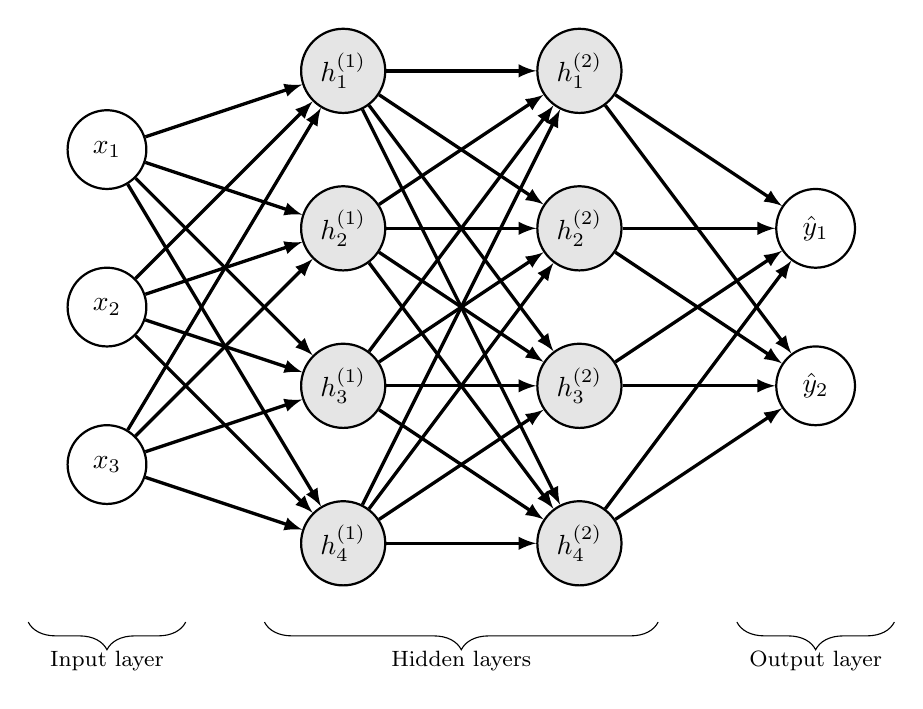
\begin{tikzpicture}[item/.style={circle,draw,thick,align=center},
itemc/.style={item,join}]
%Input Layer
\node[item, minimum size = 10mm, fill = white] (i-1) at (0, 0) {$x_1$};
\node[item, minimum size = 10mm, fill = white] (i-2) at (0, -2){$x_2$};
\node[item, minimum size = 10mm, fill = white] (i-3) at (0, -4){$x_3$};
%First Hidden Layer
\node[item, minimum size = 10mm, fill = gray!20] (h1-1) at (3, 1) {$h^{(1)}_1$};
\node[item, minimum size = 10mm, fill = gray!20] (h1-2) at (3, -1) {$h^{(1)}_2$};
\node[item, minimum size = 10mm, fill = gray!20] (h1-3) at (3,-3) {$h^{(1)}_3$};
\node[item, minimum size = 10mm, fill = gray!20] (h1-4) at (3,-5) {$h^{(1)}_4$};
%Second Hidden Layer
\node[item, minimum size = 10mm, fill = gray!20 ] (h2-1) at (6,1) {$h^{(2)}_1$};
\node[item, minimum size = 10mm, fill = gray!20 ] (h2-2) at (6,-1) {$h^{(2)}_2$};
\node[item, minimum size = 10mm, fill = gray!20 ] (h2-3) at (6,-3) {$h^{(2)}_3$};
\node[item, minimum size = 10mm, fill = gray!20 ] (h2-4) at (6,-5) {$h^{(2)}_4$};
%Outputlayer
\node[item, minimum size = 10mm, fill = white ] (o-1) at (9,-1) {$\hat{y}_1$};
\node[item, minimum size = 10mm, fill = white ] (o-2) at (9,-3) {$\hat{y}_2$};
 
% Connect neurons 
\foreach \i in {1,...,3}{
    \foreach \j in {1,...,4}{
        \draw[-latex, very thick] (i-\i) -- (h1-\j);}}
\foreach \i in {1,...,4}{
    \foreach \j in {1,...,4}{
        \draw[-latex, very thick] (h1-\i) -- (h2-\j);}}
\foreach \i in {1,...,4}{
    \foreach \j in {1,...,2}{
        \draw[-latex, very thick] (h2-\i) -- (o-\j);}}

\draw [decorate, decoration = {brace, amplitude = 10pt}, xshift = 0pt, yshift = 0pt]
    (1,-6) -- (-1,-6) node [black,midway,xshift=0cm,yshift=-0.5cm] 
    {\footnotesize Input layer};
\draw [decorate,decoration={brace,amplitude=10pt},xshift=0pt,yshift=0pt]
    (7,-6) -- (2,-6) node [black,midway,xshift=0cm,yshift=-0.5cm] 
    {\footnotesize Hidden layers};
\draw [decorate,decoration={brace,amplitude=10pt},xshift=0pt,yshift=0pt]
    (10,-6) -- (8,-6) node [black,midway,xshift=0cm,yshift=-0.5cm] 
    {\footnotesize Output layer};
\end{tikzpicture}
\label{abb:NN}
\caption{Graph representation of a neural network with two hidden layers}
\end{figure}


As a layer is constructed to use the same input for each neuron, we can use the output of a layer as input for a new layer which is exemplarily shown in Figure \ref{abb:NN}. 
A special role has the \textit{input layer}, which is the "first" layer and just contains the input variables, and the \textit{output layer}, the "last" layer which returns the prediction of the neural network. All other layers of the network are called \textit{hidden layers} as in general only input and output are observable for the network user while all the calculations that happen in between remain hidden.\\

\begin{definition}
A special activation function for the output layer is the softmax function. This is specifically used in classification tasks. Here for each of the output neurons $i=1,\cdotsc$ represents one of the $c$ possible classes. The output of the softmax function for the $i$-th neuron:
$$softmax_i(x)= \frac{e^{x_i}}{\sum_{j=1}^{c}e^{x_j}},$$
with $x=(x_1,\cdots,x_{c})\in \R^{c}$, then can be interpreted as the probability of the observation belonging to the respective class.
\end{definition}

\begin{definition}
    We now can define a fully connected neural network $f$ with architecture $(L,p)$, where $L\in \bN_0$ is the number of hidden layers and $p=(p_0,p_1,\cdots, p_L, p_{L+1}) \in\bN^{L+2}$ contains the layer sizes or widths.\\
    The input layer consists of the input vector $h^{(0)} = x = (x_1,\cdots, x_{p_0})^T\in\R^{p_0}$. \\
    For the $L$ hidden layers $l=1,\dots, L$ compute a hidden state
    $$h^{(l)}=\sigma^{(l)}( W^{(l)} * h^{(l-1)} + b^{(l)})$$
    where $W^{(l)}\in \R^{p_{l-1}\times p_l}$ is the weight matrix, $b^{(l)}\in R^{p_l}$ is the bias vector, and $\sigma^{(l)}$ is the activation function of the $l$-th layer.\\
    The output of the network is then given by 
    $$f(x)=\hat{y}= \sigma^{(o)}( W^{(o)} * h^{(L)}+b^{(o)}).$$
    with $W^{(o)}\in\R^{p_{L+1} \times p_L}$ being the output weight, $b^{(o)}\in\R$ the output bias and $\sigma_o$ the output activation function.
\end{definition}

\section{Training a neural network}
\color{red} whole section about training of a nn\\
training loss/ loss function 
SGD/batches
dropout
\color{black}

\section{RNN}
Because a neural network is defined with fixed layer sizes, especially a fixed input dimension it only allows input $x\in\R^{p_0}$.
In the marketing attribution setting, we're working with sequential data that has varying lengths for each individual customer journey. To accommodate different customer journeys and recognize that for each touchpoint the same variables are observed a recurrent approach seems fitting as they are a common approach for this type of sequential data. 
For now, we do not care about the exact time interval between two observations and rather look at the timestamps as establishing an order. The exact time points will be important for the time gate later.\\
Let $x=(x_1,\cdots,x_T)$ be one sequential observation (i.e. one customer journey) consisting of $T$ chronologically ordered observations within the sequence, i.e. customer-brand interactions and $x_t\in \R^{n}$ is a vector that collects all the information of the $t$-th touchpoint. For all touchpoints, the same $n$ features are observed, with the exact time of the touchpoint possibly being one of them.\\

RNNs continue basic neural networks to sequential usage, they can make predictions after each time step $(\{\hat{y_1},\hat{y_2}, \dots, \hat{y_T}\})$ or only after the last time step $(\{\hat{y_T}\})$ using information from all previous time steps. 
To do so a neural network $f$ with input size $n+p_{L+1}$ is trained to make calculations for each timestep but instead of only using the observations $x_t$ of this timestep one also uses the output $h_{t-1}$ of the network for the previous timestep as input. $$h_t=f(x_t,h_{t-1})$$
This output $h_{t}$ is also called \textit{hidden state} and contains all the information of  previous timesteps. The initial hidden state $h_0$ does not exist as no earlier information before $x_1$ is known, but the vector is needed for calculations. Therefore in general it simply gets initialized as a zero vector.\\
The hidden state can be viewed as the output of the network or can be used for further calculations.\\
\cite{sherstinsky-2020} gives an in-depth explanation of how to get and unroll a recurrent neural network which is visually represented in Figure \ref{abb:RNN} where $H$ can be understood as just one single layer or a whole network with multiple layers.\\
If we take RNNs further we can create even more diverse networks.
In Figure \ref{abb:differentRNN} see several different possibilities that can be realized with a recurrent neural network. Especially several recurrent layers put one after another, RNNs where not all layers are recurrent or recurrent connections that not only connect to the same but different layers.\\


\begin{figure}[h]
    \centering
\begin{tikzpicture}[item/.style={circle,draw,thick,align=center},
itemc/.style={item,on chain,join}]
 \begin{scope}[start chain=going right,nodes=itemc,every
 join/.style={-latex,very thick},local bounding box=chain]
 \path node[rectangle, rounded corners, minimum width=1.5cm, minimum height=1cm, fill=gray!20] (A0) {$H$} node[rectangle, rounded corners,minimum width=1.5cm, minimum height=1cm, fill=gray!20] (A1) {$H$} node[rectangle, rounded corners,minimum width=1.5cm, minimum height=1cm, fill=gray!20] (A2) {$H$} node[rectangle, rounded corners,minimum width=1.5cm, minimum height=1cm, xshift=2em, fill=gray!20] (AT)
 {$H$};
 \end{scope}
 \node[left=1em of chain,scale=2] (eq) {$=$};
 \node[rectangle, rounded corners, left=2em of eq, minimum width=1.5cm, minimum height=1cm, fill=gray!20, draw=black] (AL) {$H$};
 \path (AL.west) ++ (-1em,2em) coordinate (aux);
 \draw[-latex,very thick,rounded corners] (AL.east) -| ++ (1em,2em) -- (aux) 
 |- (AL.west);
 \foreach \X in {0,1,2,T} 
    {\draw[-latex,very thick] (A\X.north) -- ++ (0,2em)
    node[above,item,fill=white] (h\X) {$h_\X$};
    \draw[latex-,very thick] (A\X.south) -- ++ (0,-2em)
    node[below,item,fill=white] (x\X) {$x_\X$};}
 \draw[white,line width=0.8ex] (AL.north) -- ++ (0,1.9em);
 \draw[-latex,very thick] (AL.north) -- ++ (0,2em)
 node[above,item,fill=white] {$h_t$};
 \draw[latex-,very thick] (AL.south) -- ++ (0,-2em)
 node[below,item,fill=white] {$x_t$};
 \path (x2) -- (xT) node[midway,scale=2,font=\bfseries] {\dots};
\end{tikzpicture}
\label{abb:RNN}
\caption{Recurrent Neural Network}
\end{figure}

When training recurrent neural networks we also want to minimize the training loss and therefore we view the training loss as a function of the weights and biases. To find the the minimal training loss we now use something called \color{red} backpropagation through time (BPTT) \color{black} to calculate the gradient. The gradient now reflects the recurrent structure of the network. Because we always use the entire output of a timestep for the next calculations, where it gets multiplied with some weights, when trying to find the derivative we need to go back through all timesteps, and some of the weight matrixes are multiplied several times with themselves. This matrix multiplication can quickly result in either very small or extremely large values, i.e. exploding or vanishing gradients. which means the algorithm used to optimize the parameters can't work well because with large gradients on likely skips over the critical point where loss would be minimized and with small gradients the steps towards this critical point are too insignificant to reach them in a reasonable timeframe. \color{red}source\color{black}\\

\begin{figure}[h]
    \centering
\begin{tikzpicture}[
roundnode/.style={circle, draw=black, fill=white, very thick, minimum size=7mm},
squarednode/.style={rectangle, rounded corners, minimum width=1.5cm, minimum height=1cm, fill=gray!20, draw=black]},
explainnode/.style={rectangle, draw=black!1,text width=10em, minimum width=1.5cm, minimum height=1cm]},
]
%Nodes
\node[squarednode]      (H1)                     {$H_1$};
\node[squarednode]      (H2)       [above=of H1] {$H_2$};
\node[roundnode]        (ht)       [above=2em of H2] {$h_t$};
\node[roundnode]        (xt)       [below=1.5em of H1] {$x_t$};
\node[explainnode]  (e)            [below=1.5em of xt] {all layers are recurrent};
%recurrent layers}

%Lines
\path (H1.west) ++ (-1em,2em) coordinate (aux1);
\draw[-latex, very thick, rounded corners] (H1.east) -| ++ (1em,2em) -- (aux1) |- (H1.west);
\path (H2.west) ++ (-1em,2em) coordinate (aux2);
\draw[-latex, very thick, rounded corners] (H2.east) -| ++ (1em,2em) -- (aux2) |- (H2.west);

\draw[-latex, very thick] (xt.north) -- (H1.south);
\draw[white,line width=0.8ex] (H1.north) -- (H2.south);
\draw[-latex ,very thick] (H1.north) -- (H2.south);
\draw[white,line width=0.8ex] (H2.north) -- (ht.south);
\draw[-latex, very thick] (H2.north) -- (ht.south);

%Nodes
\node[squarednode]      (H31)       [right= 8em of H1] {$H_1$};
\node[squarednode]      (H32)       [above=of H31] {$H_2$};
\node[roundnode]        (h3t)       [above=2em of H32] {$h_t$};
\node[roundnode]        (x3t)       [below=1.5em of H31] {$x_t$};
\node[explainnode]      (e2)    [below=1.5em of x3t] {only one recurrent layer};
%only one recurrent layers}

%Lines
\path (H32.west) ++ (-1em,2em) coordinate (aux32);
\draw[-latex, very thick, rounded corners] (H32.east) -| ++ (1em,2em) -- (aux32) |- (H32.west);

\draw[-latex, very thick] (x3t.north) -- (H31.south);
\draw[white,line width=0.8ex] (H31.north) -- (H32.south);
\draw[-latex ,very thick] (H31.north) -- (H32.south);
\draw[white,line width=0.8ex] (H32.north) -- (h3t.south);
\draw[-latex, very thick] (H32.north) -- (h3t.south);

%nodes
\node[squarednode]      (H21)      [right= 8em of H31] {$H_1$};
\node[squarednode]      (H22)      [above=of H21] {$H_2$};
\node[roundnode]        (h22t)     [above=2em of H22] {$h_t$};
\node[roundnode]        (x2t)       [below=1.5em of H21] {$x_t$};
\node[explainnode]      (e3)        [below=1.5em of x2t] {recurrence between different layers};
%recurrency between different layers}

%lines
\path (H22.west) ++ (-1em,-2.5em) coordinate (aux21);
\draw[-latex, very thick, rounded corners] (H22.east) -| ++ (1em,-2.5em) -- (aux21) |- (H21.west);
\draw[-latex, very thick] (x2t.north) -- (H21.south);
\draw[white,line width=0.8ex] (H21.north) -- (H22.south);
\draw[-latex ,very thick] (H21.north) -- (H22.south);
\draw[white,line width=0.8ex] (H22.north) -- (h22t.south);
\draw[-latex, very thick] (H22.north) -- (h22t.south);

\end{tikzpicture}
\label{abb:differentRNN}
\caption{Different possibilities for RNNs}
\end{figure}


\cite{hochreiter-1997} introduce Long-Short Term Memory (LSTM) Networks to solve this by restricting the information that is remembered from previous time steps 
\color{red}appendix LSTM?\color{black}.


\section{Gated Recurrent Units}
Gated recurrent units (GRU) as proposed by \cite{cho-2014} are a simplification of LSTM cells. They have the advantage of using less memory space and fewer calculations while retaining the same benefits of generally leading to improved performance and not having the exploding/vanishing gradient problem that LSTMs were created for.\\
A gated recurrent unit corresponds to one layer of a RNN. We sometimes will use the term GRU cell to especially refer to a single unit/layer and differentiate it from a whole network. \\
To define gated recurrent units we need the Hadamard product:
\begin{definition}
    The Hadamard Product $\odot$ is defined as an operation between two matrices of the same dimension as elementwise multiplication. Let $A,B\in \R^{n\times m}$ with $n,m \in \bN$, then 

\begin{align*}
 A \odot B= && \begin{pmatrix}
a_{11} & a_{12} & \cdots & a_{1m} \\
\vdots & \vdots & \ddots & \vdots \\
a_{n1} & a_{n2} & \cdots & a_{nm}
\end{pmatrix} 
\odot
\begin{pmatrix}
b_{11} & b_{12} & \cdots & b_{1m} \\
\vdots & \vdots & \ddots & \vdots \\
b_{n1} & b_{n2} & \cdots & b_{nm} 
\end{pmatrix} \\ = 
&& \begin{pmatrix}
a_{11}*b_{11} & a_{12}*b_{12} & \cdots & a_{1m}*b_{1m} \\
\vdots & \vdots & \ddots & \vdots \\
a_{n1}*b_{n1} & a_{n2}*b_{n2} & \cdots & a_{nm}*b_{nm}
\end{pmatrix}
\end{align*}

\end{definition}

\begin{definition}
    We define the gated recurrent units as proposed in \cite{cho-2014} with two gates. Assume $x_t \in \R ^{p_0}$\\
    A reset gate:
    \begin{align} \label{eq:resetgate}
        r_t= \sigma_r\left(W_{rx} x_t + W_{rh} h_{t-1} + b_r\right)
    \end{align}
    and an update gate:
    \begin{align} \label{eq:updategate}
    z_t= \sigma_z\left(W_{zx} x_t + W_{zh} h_{t-1} + b_z\right) \end{align}
    with $\sigma_r,\sigma_z$ the sigmoid activation function $\sigma(x)=\frac{1}{1+\exp{-x}}$. Both gates return values in $[0,1]$ in each position, 0 meaning the gate for this variable is fully closed, and 1 that it is open.\\
    We then get a hidden state candidate
    \begin{align} \label{eq:candidate}
    \Tilde{h}_t=\sigma_h(W_{hx} x_t+W_{hh} (r_t\odot h_{t-1} + b_h )
    \end{align}
    and finally the hidden state is
    \begin{align} \label{eq:hiddenstate}
    h_t=z_t\odot h_{t-1} +(\mathds{1} - z_t)\odot \Tilde{h}_t
    \end{align}
    which also is the output for this timepoint.
    \color{red} 1 sollte $(1,\cdots,1) \in \R^{p_t}$ Vektor \\ \color{black} It is obvious that when the update gate returns a value close to 0,  it ignores the previous hidden state on the other hand if it is close to 1 the current information is ignored and only previous information is used for the new hidden state.
\end{definition}

\section{Time gate}
In this thesis, an additional time gate which \cite{neil-2016} introduced for LSTM cells creating a so-called phased-LSTM will be added to the gated recurrent units to form a phased GRU network. 

\begin{definition}  The time gate \cite{neil-2016} proposed uses the timestamp $t$ of the current input and calculates the openness of the time gate $k_t$ which then controls how the output of the layer gets updated. 
It uses three different parameters for the calculation, which can be learned during the training phase. 
The time gate opens and closes periodically, so first calculate an auxiliary variable $\varphi_t$, to determine the phase of the current cycle.
 $$\varphi_t=\frac{(t-s) \mod \tau}{\tau} \in [0,1)$$
It uses $\tau$, which controls the real-time period and $s$ phase shift of the oscillation.
Furthermore, there is the parameter $r_{on}$ which determines the ratio of the duration of the open phase to the full period.\\    
Then use this to calculate the time gate
\begin{align}
    k_t= \begin{cases} \frac{2\varphi_t}{r_{on}}, & \text{if } \varphi_t< \frac{1}{2} r_{on}\\
    2- \frac{2\varphi_t}{r_{on}}, & \text{if }  \frac{1}{2} r_{on} < \varphi_t < r_{on}\\
    \alpha\varphi_t, &\text{otherwise} \end{cases}
    \label{eq:time gate}
\end{align}
\end{definition}

\begin{explanation}
The time gate \ref{eq:time gate} has two phases, the open and the close phase.
In the first half of the open phase ($\varphi_t<\frac{1}{2}r_{on}$) the time gate gradually opens from $0$ to $1$. and closes back down from $1$ to $0$ in the second half ($\frac{1}{2} r_{on} < \varphi_t < r_{on}$).
While $\varphi_t \geq r_{on}$ the gate is in its closed phase, where instead of setting $k_t = 0$ and cutting off all information only a small portion ($\alpha<<1$) of the current state is let through. This way important information can still make an impact later on and is not completely lost, while the remaining information is reduced enough for the time gate to make sense. 
A similar thing is done with leaky ReLu instead of a strict ReLu.
\end{explanation}


Now a phased GRU cell can be defined by extending the basic GRU cell.
\begin{definition}
    We can use \ref{eq:resetgate} \ref{eq:updategate} and \ref{eq:candidate}  from the GRU cell.
    Instead of the hidden state
    \begin{align}
        \Bar{h}_t= z_t\odot h_{t-1} +(\mathds{1}-z_t)\odot \Tilde{h}_t
    \end{align}
    is another hidden state candidate and 
    \begin{align}
        h_t =  k_t \odot\Bar{h}_t + (\mathds{1}-k_t)\odot h_{t-1}
    \end{align}
    is the actual hidden state 
\end{definition}

\begin{figure}[h]
    \centering
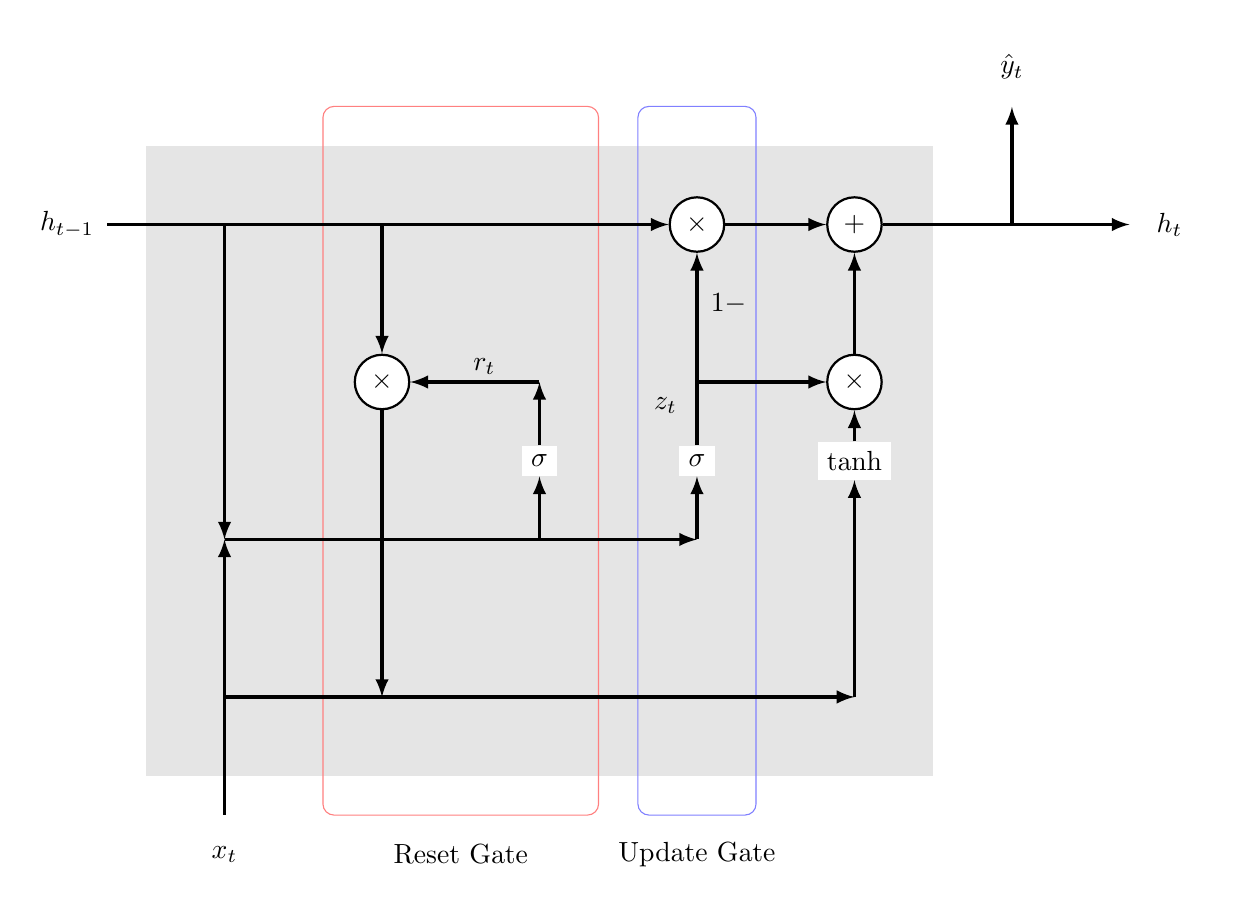
\begin{tikzpicture}[item/.style={circle,draw,thick,align=center},
itemc/.style={item,join}]
%Input Layer
\node[rectangle, minimum width = 10cm,minimum height=8cm, fill = gray!20] (GRUcell) at (6, 5) {};
\node[rectangle, minimum size = 10mm, fill = gray!20] (minus) at (8.4, 7) {$1-$};
\node[rectangle, minimum size = 10mm, fill = gray!20] (rt) at (5.3, 6.2) {$r_t$};
\node[rectangle, minimum size = 10mm, fill = gray!20] (zt) at (7.6, 5.7) {$z_t$};

\node[rectangle, minimum size = 10mm, fill = white] (ug) at (8, 0){Update Gate};
\node[rectangle, minimum size = 10mm, fill = white] (rg) at (5, 0){Reset Gate};

\node[rectangle, rounded corners, minimum width = 3.5cm, minimum height=9cm, draw=red!50] (updategate) at (5,5) {};
\node[rectangle, rounded corners, minimum width = 1.5cm, minimum height=9cm, draw=blue!50] (resetgate) at (8,5) {};

\node[rectangle, minimum size = 10mm, fill = white] (xt) at (2, 0){$x_t$};
\node[rectangle, minimum size = 10mm, fill = white] (htmo) at (0, 8){$h_{t-1}$};
\node[rectangle, minimum size = 10mm, fill = white] (ht) at (14, 8) {$h_t$};
\node[rectangle, minimum size = 10mm, fill = white] (yt) at (12, 10) {$\hat{y}_t$};
\node[item, fill = white] (p) at (10, 8) {$+$};
\node[item, fill = white] (m1) at (10, 6) {$\times$};
\node[item, fill = white] (m2) at (8, 8) {$\times$};
\node[item, fill = white] (m3) at (4, 6) {$\times$};
\node[rectangle, fill = white] (sig1) at (6, 5) {$\sigma$};
\node[rectangle, fill = white] (sig2) at (8, 5) {$\sigma$};
\node[rectangle, fill = white] (tanh) at (10, 5) {$\tanh$};
\draw[latex-,very thick] (m2.west) -- (htmo.east);
\draw[latex-,very thick] (2,4) -- (xt.north);
\draw[latex-,very thick] (2,4) -- (2, 8);
\draw[latex-,very thick] (8,4) -- (2, 4); 
\draw[latex-, very thick] (4,2) -- (m3.south);
\draw[latex-,very thick] (m3.north) -- (4,8);
\draw[-latex,very thick] (2,2) -- (10,2);
\draw[-latex,very thick] (10,2) -- (tanh.south);
\draw[-latex,very thick] (tanh.north) -- (m1.south);
\draw[-latex,very thick] (8,4) -- (sig2.south);
\draw[-latex,very thick] (6,4) -- (sig1.south);
\draw[-latex,very thick] (sig2.north) -- (m2.south);
\draw[-latex,very thick] (8,6) -- (m1.west);
\draw[-latex,very thick] (sig1.north) -- (6,6);
\draw[-latex,very thick] (6,6) -- (m3.east);
\draw[-latex,very thick] (m2.east) -- (p.west);
\draw[-latex,very thick] (p.east) -- (ht.west);
\draw[-latex,very thick] (m1.north) -- (p.south);
\draw[-latex,very thick] (12,8) -- (yt.south);


\end{tikzpicture}
\label{abb:GRU}
\caption{Gated Recurrent Unit}
\end{figure}


\color{red}
    one gru cell corresponds to one layer, multiple layer are possible \\
    prediction does not need to happen each time step.\\
    For the MTA model two GRU layers and a softmax layer prediction only after final timestep $\hat{y}=(\hat{y}_0, \hat{y}_1)^T\in [0,1]^2$ with $\hat{y}_0$ predicted probability for no conversion, $\hat{y}_1$ predicted probability for conversion 
\color{black}

This concludes the conversion predictor
